\section{Quality assurance}

Verification is an internal characteristic (we need to check if we are building the software right).
Validation is an external characteristic (we need to check if we are building the right software).

\begin{definition}[\textit{Quality assurance }]
    Quality assurance define policies and processes to achieve quality. 
\end{definition}
Quality may refer to: 
\begin{itemize}
    \item Absence of defects (or bugs).
    \item Absence of other issues that prevent the fulfillment of non-functional requirements or the degradation of some software qualities. 
    \item External qualities (e.g.,performance,availability). 
    \item Internal qualities (e.g.,maintainability). 
\end{itemize}

\begin{definition}[\textit{Failure}]
    The failure termination of the ability of a product to perform a required function or its inability to perform within previously specified limits.
    The failure can also be seen as an event in which a system or system component does not perform a required function within specified limits.
\end{definition}
\begin{definition}[\textit{Fault}]
    Fault is the manifestation of a defect. 
\end{definition}
\begin{definition}[\textit{Defect}]
    The defect is an imperfection or deficiency in a program (e.g., function should always return a positive value, but returns a negative value in this case). 
\end{definition}
\begin{definition}[\textit{Error}]
    An error is a human action that introduced an incorrect result. 
\end{definition}
\begin{figure}[H]
    \centering
    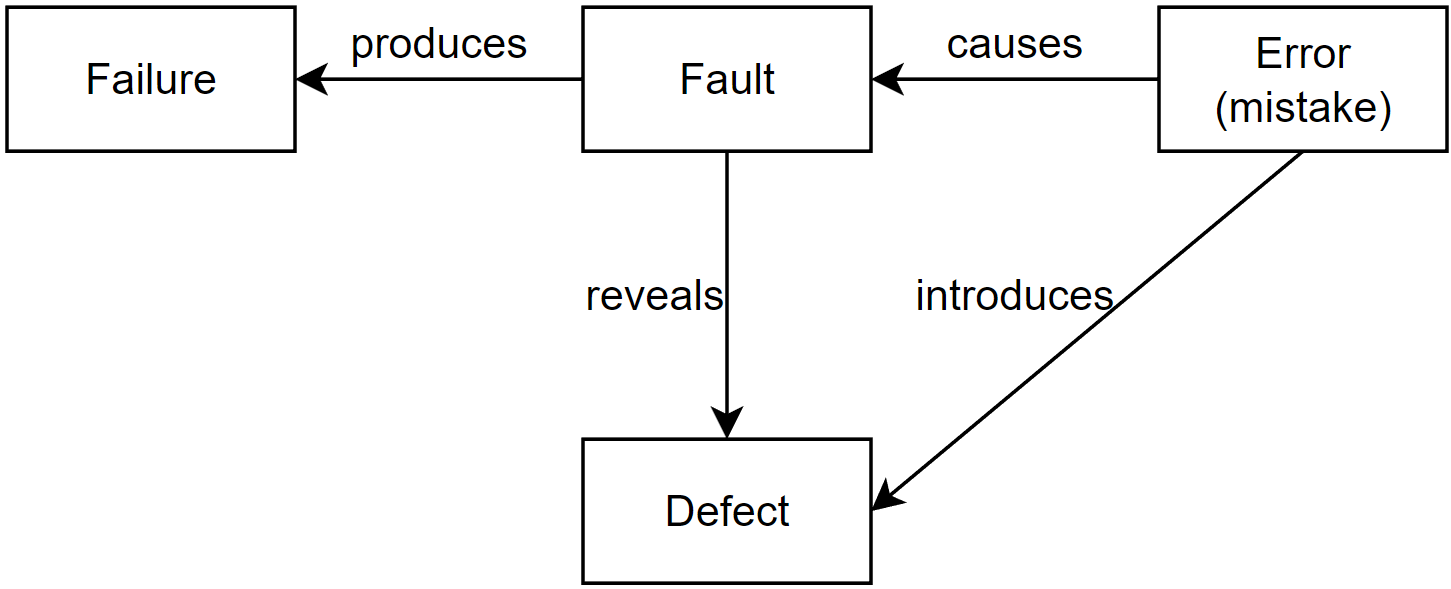
\includegraphics[width=0.6\linewidth]{images/ver.png}
    \caption{Failure, fault, defect, and errors}
\end{figure}

Zero defect software practically impossible to achieve, so careful and continuous quality assurance is needed. 
Ideally, every artifact shall be subject of quality assurance.
Even the verification artifacts must be verified. 

\paragraph*{Structural engineering and software engineering}
In structural engineering we may have a request to build a bridge. 
Suppose that it shall support heavy trucks (40 tons). 
To test this requirement we can for example load the bridge with 50 tons. 
In this case we have that one test covers infinite cases. 

In software engineering we may have a request to build a program.
Since programs do not display a continuous behavior, verifying a program for a single data point does not tell us anything about other points. 

As a result, depending on the level of the implementation we have to use different verification techniques: 
\begin{figure}[H]
    \centering
    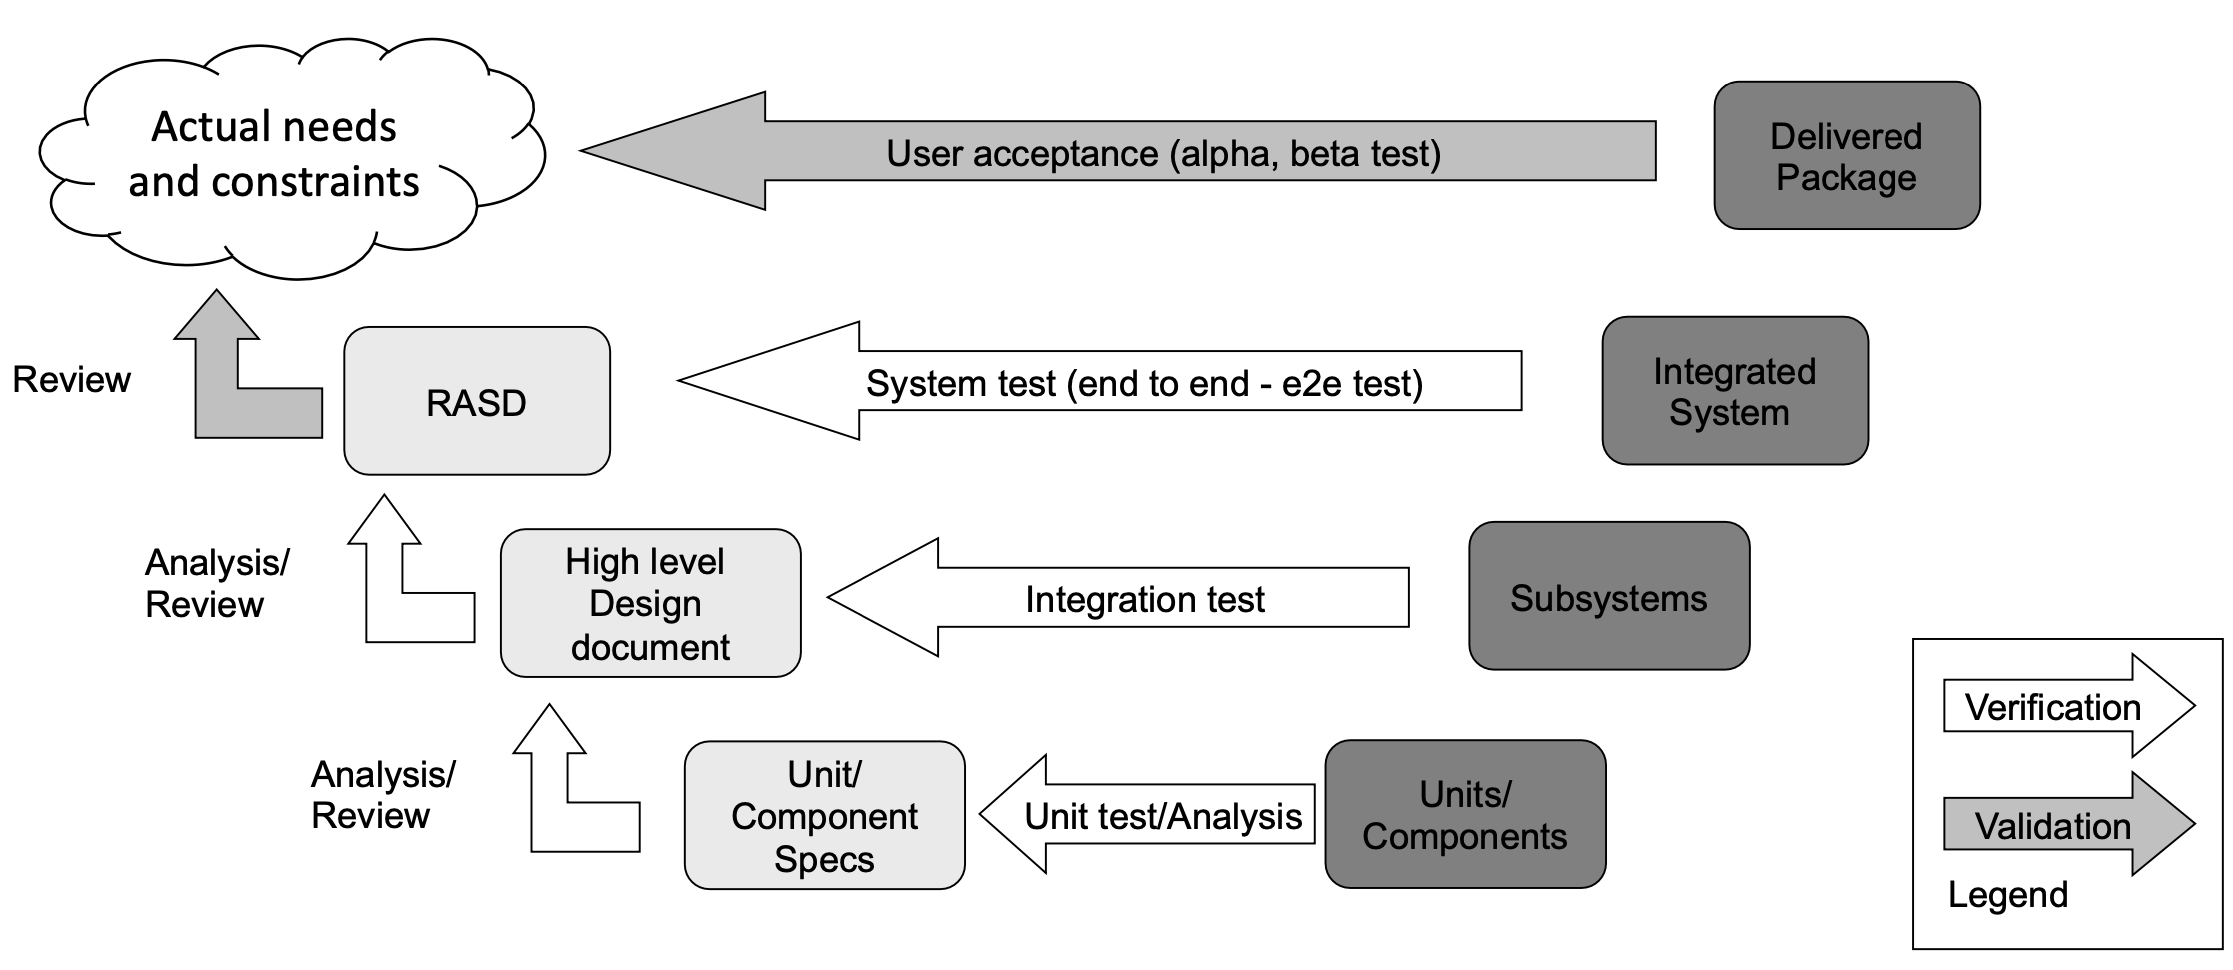
\includegraphics[width=0.75\linewidth]{images/ver1.png}
\end{figure}

\paragraph*{Possible approaches}
To test the program we have two main approaches: 
\begin{itemize}
    \item \textit{Static analysis}: this type of analysis is done on source code without execution. 
        Note that the properties are dynamic. 
    \item \textit{Dynamic analysis}: this type of analysis, also called testing, is done by executing the sources (usually by sampling). 
        In this analysis we check the actual behavior of the program compared to an expected one. 
\end{itemize}


SLIDE 17